%% A3 CHIA Hackathon 2026 — 4-page paper.
%% Format required by the CFP: 4 pages, 2-column ACM/IEEE style, PDF.
%% Template: ACM acmart, sigconf. `nonacm` drops the ACM copyright/DOI footer.
\documentclass[sigconf,nonacm]{acmart}

\setlength{\emergencystretch}{1.5em}

\begin{document}

\title{A GPU-Accelerated DREAMPlace/OpenROAD Evaluator Node for CHIA}
\subtitle{Multi-Backend, Cached Evaluation, and Noise-Aware Agentic Search}

\author{Kaviprashanna Krishnamoorthy}
\affiliation{%
  \institution{Independent Researcher}
  \country{India}}
\email{kavinittrichy@gmail.com}

\begin{abstract}
An agent that tunes physical design needs feedback from routed layouts, not
from the placer's own cost function. We present a reusable CHIA evaluator node that
places designs with DREAMPlace on the GPU, hands the placement back to
OpenROAD-flow-scripts, and always closes the loop through real routing. The
same interface also drives LibreLane, where a small sky130 design passes Magic
DRC and Netgen LVS signoff. On gcd, DREAMPlace's wirelength proxy is
weakly anti-correlated with routed wirelength (Spearman $-0.29$), while the
global-route estimate tracks it almost perfectly ($+0.99$), so we rank candidates with a proxy/global-route/route funnel.
Because routing amplifies tiny placement differences, a search result counts
only if it holds on held-out seeds and beats the default knobs, routed on the
same seeds, by more than $2\sigma$. We
compare against stock ORFS on gcd, tinyRocket and Ariane133, and against AutoDMP
on tinyRocket. On tinyRocket, knob search shortens routed wirelength by up to 4.4\%
with every route DRC-clean, while AutoDMP's best trial has 159 DRC violations.
The remaining results are negative: an LLM proposer is indistinguishable from
random search, stock ORFS keeps better setup timing on tinyRocket and Ariane133,
and our end-to-end flow is slower on both.
\end{abstract}

\keywords{physical design, placement, OpenROAD, DREAMPlace, LLM agents,
CHIA, design-space exploration}

\maketitle

%% =====================================================================
\section{Introduction}
\label{sec:intro}
A placement that looks good on the placer's own objective can route badly.
Wirelength proxies reward dense placements, and density costs routability.
An agent that tunes a placer against its proxy can therefore optimize the wrong
thing without its designer noticing. CHIA~\cite{chia} makes it easy to put an
agent in the loop. We ask what that loop must measure for the agent's feedback
to mean anything, and what the agent then learns.

Our answer is an evaluator node that carries every candidate through real
routing and measures how much of any improvement is noise. We report the
outcome whichever way it falls. Our contributions are:
\begin{itemize}
  \item A pluggable evaluator contract (\texttt{EvalRequest}/\texttt{EvalResult})
    with per-experiment backend selection, GPU/CPU-split place and route CHIA
    functions, and content-addressed caching with provenance (\S\ref{sec:node}).
  \item An ORFS/OpenROAD backend (NanGate45) that splices DREAMPlace GPU global
    placement into stock ORFS through a components-only DEF, checks that
    OpenROAD does not re-place it, and runs through detailed routing.
  \item A LibreLane backend (sky130) with the same DREAMPlace splice, reaching
    Magic DRC\,=\,0 and Netgen LVS\,=\,0 on \texttt{spm}, and LVS\,=\,0 on a design
    with two SRAM macros.
  \item A three-tier proxy/global-route/route funnel, justified by a measured
    rank-correlation study (\S\ref{sec:protocol}, \S\ref{sec:results}).
  \item A noise-aware protocol (seed-lottery baseline, held-out seeds, a
    $2\sigma$ rule) comparing an LLM proposer with random search on routed
    results, alongside single-run AutoDMP~\cite{autodmp}, stock RePlAce and
    Hammer-wrapped OpenROAD baselines.
\end{itemize}

%% =====================================================================
\section{Background}
\label{sec:background}
DREAMPlace~\cite{dreamplace} casts analytical global placement as neural-network
training in PyTorch, which gives large GPU speedups over RePlAce. AutoDMP~\cite{autodmp}
wraps DREAMPlace in multi-objective Bayesian optimization for macro placement;
we use it only as a baseline. OpenROAD~\cite{openroad} and its
flow scripts (ORFS~\cite{orfs}) form an open RTL-to-GDS flow. LibreLane~\cite{librelane}
is an open flow with Magic/Netgen signoff on sky130. CHIA~\cite{chia} is a
framework for agentic hardware design; our evaluator runs as CHIA functions.

%% =====================================================================
\section{The Evaluator Node}
\label{sec:node}
\begin{figure*}[t]
  \centering
  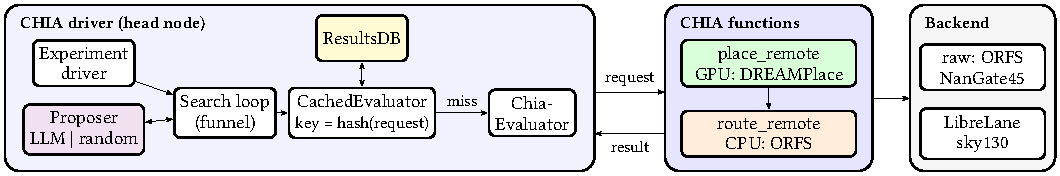
\includegraphics[width=\textwidth]{tikz/fig_overview.pdf}
  \Description{Block diagram: the CHIA driver (experiment driver, search loop, proposer, cached evaluator with results database, CHIA evaluator) exchanges requests and results with CHIA functions on Ray workers (GPU placement, CPU routing), which run the ORFS or LibreLane backend.}
  \caption{The evaluator node in CHIA. The driver proposes, caches and
  deduplicates requests. Placement runs as a GPU CHIA function and routing as a
  CPU-only one on the same VM. The flow backend is chosen per experiment.}
  \label{fig:overview}
\end{figure*}
\paragraph{Contract and backends.}
Fig.~\ref{fig:overview} shows the node. An \texttt{EvalRequest} names a design, technology, placer knobs, seed, stage
(\texttt{proxy}, \texttt{grt} or \texttt{route}) and a toolchain fingerprint.
An \texttt{EvalResult} carries the placer's half-perimeter wirelength (HPWL, the
proxy), global-route and routed wirelength (WL), worst and total negative slack
(WNS/TNS), power, area, design-rule-check (DRC) violation count and provenance. The flow engine is chosen per
experiment by the evaluator's configuration: \texttt{raw}
(ORFS/OpenROAD, NanGate45) or \texttt{librelane} (sky130). Callers (the
search loop and experiment driver) are backend-agnostic. All search experiments
in this paper use the ORFS backend; the LibreLane backend was validated with
individual evaluations. Placement and routing are separate CHIA functions. Only
placement reserves a GPU, so CPU-bound routing never holds one. As host
flow we also tried Hammer-wrapped OpenROAD, hand-tuned toward ORFS. On gcd it is
26.3\% longer in WL (5593 vs.\ 4429\,$\mu$m) and has about 2$\times$ worse WNS
($-0.32$ vs.\ $-0.162$\,ns) at equal power (6.34 vs.\ 6.33\,mW). On aes it fails
legalization (DPL-0038), so we kept direct ORFS integration.

\paragraph{GPU placement splice.}
Stock ORFS runs to IO placement (stage 3\_2) and, after port buffering, dumps
a DEF layout file. DREAMPlace places it on the GPU, and we read the result back
from a \emph{components-only} DEF with \texttt{read\_def -incremental}.
Importing the full DEF instead re-reads the pins and later aborts detailed
routing (DRT-0302). ORFS then continues unmodified: resize, OpenDP
legalization, clock-tree synthesis (CTS), global and detailed
routing, and final reports. A splice is only valid if the host flow does not
silently re-run its own placer over ours, so every result records two checks.
First, OpenROAD's global placer prints nothing in stage 3\_3, where ORFS
normally runs it (zero \texttt{GPL-} log lines). Second, OpenDP legalization moves
cells by only 1.4\,$\mu$m on average on tinyRocket, so the final placement is
DREAMPlace's, snapped to legal sites. Optionally, DREAMPlace also legalizes
and runs its GPU detailed placer, ABCDPlace, before the handoff. On
tinyRocket this cuts OpenDP's average displacement from 1.4 to 0.3\,$\mu$m but
changes routed WL by only 0.4\% and WNS by 8\,ps (one run each), so the default hands off
global placement only.

\paragraph{Determinism, provenance, caching.}
On gcd, repeating an identical request gives bit-identical WL, WNS, TNS, power
and area, and 2 versus 8 OpenROAD threads also agree. On tinyRocket, one request
routed with place and route as separate CHIA functions (split mode) and
as one function differed by 0.07\% in WL, far below seed noise
(\S\ref{sec:protocol}). The request
identity is therefore a hash of design, technology, knobs, seed, stage and
toolchain fingerprint (image digest, DREAMPlace commit, device and GPU
architecture). A \texttt{CachedEvaluator} replays successful results for known
identities. To test the cache, we replayed two finished experiment databases
against an inner evaluator that aborts if called. All 804 (gcd) and 201
(tinyRocket) successful identities resolved from cache with zero
re-evaluations; the live runs had already served 133 and 29 cache hits. A
fresh mock-evaluator experiment, run and replayed by the released code, resolves 113/113
identities the same way.

\paragraph{Signoff backend.}
On sky130, the LibreLane backend with DREAMPlace placement reaches Magic DRC\,=\,0
and Netgen layout-versus-schematic (LVS)\,=\,0 on \texttt{spm} (routed WL 6361\,$\mu$m, WNS\,=\,0). On
\texttt{test\_sram\_macro}, with two SRAM macros, LVS is 0 but 532 DRC
violations remain, all from a single rule, \texttt{nwell.4}. NanGate45 has
no signoff deck, so ``DRC'' elsewhere in this paper means detailed-route
violations.

\paragraph{Reuse beyond this flow.}
Proposers and evaluators are pluggable. Any proposer implementing
\texttt{propose(history,\,n)}, such as a Bayesian-optimization one, runs in the
same search loop; the LLM proposer has adapters for Gemini, OpenAI-compatible
APIs, Anthropic and CHIA's own LLM calls. Any evaluator implementing
\texttt{evaluate(EvalRequest)} gets caching, the funnel and the noise protocol,
and a mock evaluator runs the full driver without EDA tools for our tests. The
rank-correlation study behind the funnel is a separate command, to be rerun on
a new design or knob range before the funnel is trusted there.

%% =====================================================================
\section{Evaluation Protocol}
\label{sec:protocol}
\begin{figure*}[t]
  \centering
  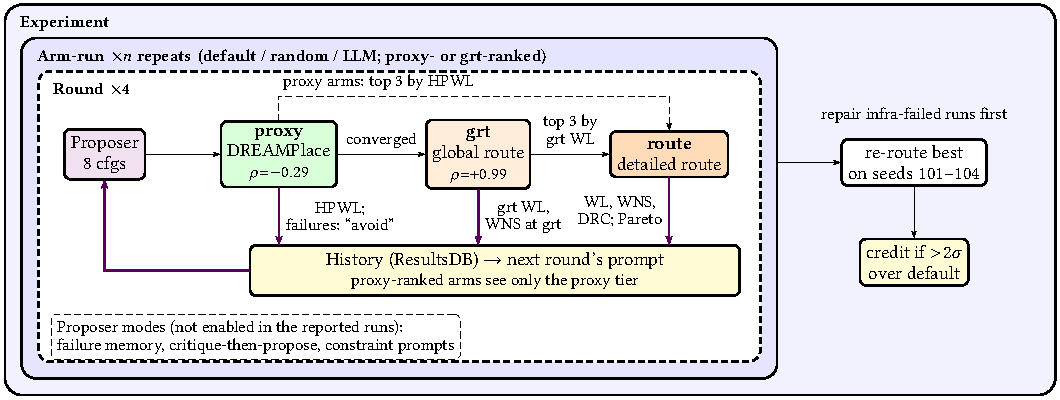
\includegraphics[width=\textwidth]{tikz/fig_protocol.pdf}
  \Description{Nested diagram: an experiment contains n repeated arm-runs, each of four search rounds. In a round the proposer's candidates pass the proxy, grt and route tiers (proxy-ranked arms skip grt and route the top 3 by HPWL). Every tier writes results into a history: HPWL and failures from the proxy, grt wirelength and WNS from global route, routed wirelength, WNS, DRC and the Pareto set from detailed route. The history becomes the next round's prompt. A dashed box lists three proposer modes not enabled in the reported runs: failure memory, critique-then-propose and constraint prompts. Afterwards each arm-run's best configuration is re-routed on held-out seeds and credited only if it beats the default by more than 2 sigma.}
  \caption{Evaluation protocol as nested loops. Each round, the proposer's
  candidates pass the tiers of one evaluator pipeline (green: GPU, orange: CPU);
  non-converged candidates stop at the proxy tier at no routing cost. Every
  tier feeds the history that forms the next round's prompt (purple); the
  proxy-only arm sees only the proxy tier. After search, each arm-run's best
  configuration is re-routed on held-out seeds and credited only if it beats
  the default by more than $2\sigma$. The random-search arms in
  Table~\ref{tab:results} ran only one round per repeat.}
  \label{fig:protocol}
\end{figure*}
\paragraph{Search loop.}
An \emph{arm} pairs a proposer (default, random or LLM) with a feedback tier;
each of its $n$ repeats is an \emph{arm-run}. Each round, the proposer emits a batch of knob settings. All reported experiments
search five DREAMPlace knobs: target density, density weight, wirelength
smoothing $\gamma$, stop overflow and learning rate. Their ranges are limited to
the region where DREAMPlace converges: 60/60 configurations converge there,
and only 33/160 do over wide ranges. The code exposes four more knobs: the global-placement iteration cap
(700--2000), the density-weight update period (1--4), sub-iterations per step
(1--2) and density-grid resolution (automatic to 512). One ablation gave the LLM
these extra knobs and added TNS, power, area, and DREAMPlace's iteration count
and final overflow to its feedback. It came within noise of the five-knob arm ($-1.3\%$ routed WL), so we
do not report it further. The random proposer samples uniformly within the same
ranges (log-uniformly for density weight and learning rate).

The LLM proposer (Gemini 3.1 Pro preview) makes one JSON-mode call per round.
Its prompt holds a task description, the knob table (ranges, defaults, log
scaling) and its own history. The history lists its 12 best routed candidates,
each with knobs, routed WL, WNS, DRC and a score
$\mathrm{WL}\cdot(1+10\,|\mathrm{WNS}^-|+0.01\,\mathrm{DRC})$, and up to eight
more routed candidates on the Pareto front of WL, WNS, power, area and DRC. It
also lists the best global-routed candidates with their estimated WL and WNS at
global route, a few proxy-only candidates with HPWL, and the latest rejected or
failed candidates with their errors, labeled as regions to avoid. The LLM
returns a short rationale and exactly one batch of knob settings. We clamp these
to the knob ranges and fill missing or malformed candidates from the random
proposer. The proxy-only ablation sees only HPWL and proxy-stage failures.
Three optional modes (dashed in Fig.~\ref{fig:protocol}; off in all reported
runs) add hints on which knob changes fixed a failure in earlier runs, a
critique of the history before proposing, or design constraints (clock period,
utilization, PPA priorities, tunable knobs) to the prompt.

\paragraph{Funnel.}
Fig.~\ref{fig:protocol} shows the funnel and the protocol together. Every candidate is placed (the \emph{proxy} tier). In the global-route arms,
converged candidates are ranked by global-route estimate (\emph{grt}); in the
proxy-only arms, by HPWL. Only the top few pay for detailed routing
(\emph{route}). A cheap tier only has to \emph{order} candidates for the next
tier, so we judge tiers by rank correlation with routed wirelength, not by
absolute error.

\paragraph{Noise.}
The flow is deterministic, but routing amplifies tiny placement differences.
Five DREAMPlace seeds of the default configuration on gcd give routed WL with
$\sigma \approx 3\%$ (range 8\%). Each arm-run's best configuration is therefore
re-routed on held-out seeds that search never saw. It is credited only if its held-out mean beats the \emph{seed-lottery
baseline}, the default configuration routed on the same seeds, by more than
$2\sigma$, where $\sigma$ is the default's seed-to-seed spread in routed WL,
measured per design.
The driver's \texttt{repair} mode detects arm-runs invalidated by
infrastructure failures and re-runs them.

%% =====================================================================
\section{Results}
\label{sec:results}
\paragraph{Proxy vs.\ route (gcd).}
We routed 60 converged configurations sampled across the knob box. Routed WL
spans 51\% of its mean, far above seed noise. DREAMPlace's HPWL ranks them with
Spearman $\rho=-0.29$ ($p=0.023$) and a top-3 recall of 0. The global-route
estimate reaches $\rho=+0.99$ and a top-3 recall of 1.0. The mechanism is
density: higher target density lowers HPWL ($\rho=-0.83$) but raises routed WL
($+0.46$). Fig.~\ref{fig:scatter} shows the scatter.

\begin{figure}[t]
  \centering
  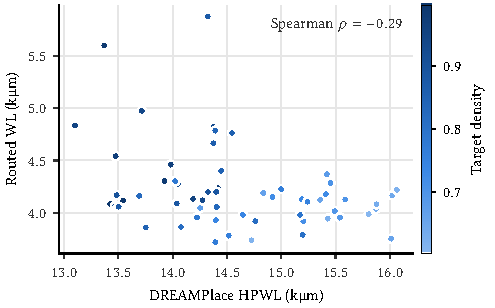
\includegraphics[width=\columnwidth]{fig_proxy_vs_routed.pdf}
  \Description{Scatter of 60 gcd placements: DREAMPlace HPWL on x, routed wirelength on y, colored by target density; points trend slightly downward.}
  \caption{DREAMPlace HPWL vs.\ routed wirelength for 60 gcd configurations.
  Higher target density (darker) lowers HPWL but raises routed WL, so the
  placer's proxy ranks configurations the wrong way ($\rho=-0.29$).}
  \label{fig:scatter}
\end{figure}

\paragraph{Search: LLM vs.\ random.}
On gcd (734 cells), no arm clears $2\sigma$ over the default, because gcd's
default knobs leave little headroom. On tinyRocket (two macros), all arm-runs were
re-routed on the same four held-out seeds (Table~\ref{tab:results}). Against the
default's spread on those seeds ($\sigma=2.0\%$), random search ($-4.3\%$) and
the proxy-only LLM ($-4.4\%$) clear $2\sigma$. The LLM with global-route
feedback ($-2.8\%$) does not. Compared directly with random search, its routed
WL differs by $+1.47\%$ (LLM longer), within two standard errors
($2\,\mathrm{SE}=2.9\%$): the two cannot be distinguished. Random search ran
one round per repeat and the LLM four, but in 5 of 6 LLM repeats the best
configuration was already found in round~1, so the budgets are effectively
matched (the sixth, a proxy-only repeat that failed entirely on
infrastructure, is excluded from Table~\ref{tab:results}). Every routed tinyRocket result, in search and validation, has 0 DRC.

\paragraph{Baselines on tinyRocket and gcd.}
We ran AutoDMP through a Bookshelf conversion, outside its tested setup. Its
best trial routes to 540{,}456\,$\mu$m with 159 DRC violations
(Fig.~\ref{fig:floorplans}). That trial's
final report aborts on a VDD connectivity check (PSM-0069), so no timing
report is available, and its detailed route took 5\,h\,06\,min vs.\ under an
hour for each of ours. Stock RePlAce, run from the same pre-placement checkpoint, is DRC-clean
at 510{,}731\,$\mu$m with WNS $-0.122$\,ns. Our held-out arm means are shorter
(best 479{,}451\,$\mu$m) but have worse setup timing (WNS $-0.20$ to
$-0.27$\,ns). On gcd, WNS is equal ($-0.161$ vs.\
$-0.162$\,ns) and all five of our seeds route shorter (3896--4256\,$\mu$m) than
stock's single run (4429\,$\mu$m).

\begin{figure}[t]
  \centering
  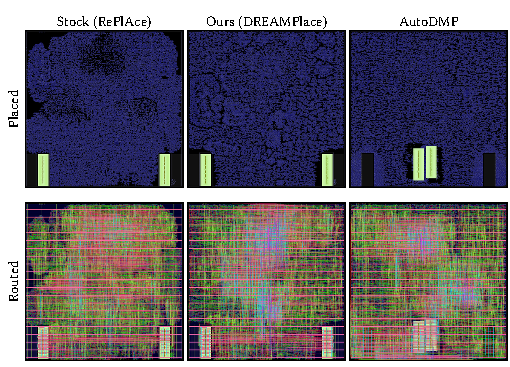
\includegraphics[width=\columnwidth]{fig_tinyrocket_floorplans.pdf}
  \Description{Six OpenROAD renders of tinyRocket: placed and routed layouts for stock RePlAce, our DREAMPlace handoff and AutoDMP. AutoDMP places both macros at the lower centre; the others keep them at the lower corners.}
  \caption{tinyRocket placed (top) and routed (bottom): stock RePlAce, our
  DREAMPlace handoff (default knobs, one seed) and AutoDMP's best trial. AutoDMP
  moves both macros to the lower centre, and its route has 159 DRC violations
  vs.\ 0 for the other two.}
  \label{fig:floorplans}
\end{figure}

\begin{table}[t]
  \caption{Routed results. tinyRocket arms: mean over 4 held-out seeds, $n$
  repeats per arm. Baselines: single run. Last row: gcd host-flow check (\S\ref{sec:node}).}
  \label{tab:results}
  \small
  \begin{tabular}{@{}lrrr@{}}
    \toprule
    tinyRocket (NanGate45) & WL ($\mu$m) & vs.\ def. & DRC \\
    \midrule
    Default config, seed lottery & 501{,}687 & --- & 0 \\
    Random, grt feedback ($n{=}2$) & 480{,}370 & $-4.25\%$ & 0 \\
    LLM, grt feedback ($n{=}3$) & 487{,}449 & $-2.84\%$ & 0 \\
    LLM, proxy only ($n{=}2$) & 479{,}451 & $-4.43\%$ & 0 \\
    Stock ORFS (RePlAce) & 510{,}731 & & 0 \\
    AutoDMP, best trial & 540{,}456 & & 159 \\
    \midrule
    gcd: direct ORFS / Hammer & 4429 / 5593 & & 0 / 0 \\
    \bottomrule
  \end{tabular}
\end{table}

\paragraph{Runtime.}
A faster placer does not make a faster flow. We timed every stage of tinyRocket
on one laptop (RTX 3060, default knobs, one run each), with DREAMPlace
legalization and detailed placement enabled. Our placement stage,
including the DEF dump and import, takes 21.8\,s vs.\ 32.2\,s for RePlAce
(DREAMPlace itself: 6.6\,s), but the downstream stages take 1.39$\times$ longer
(667 vs.\ 479\,s). Resize inserts 446 buffers vs.\ 22, CTS takes twice as
long, and detailed routing needs 12 iterations instead of 5. End to end, our flow
is 1.29$\times$ slower (791 vs.\ 611\,s; 1.14$\times$ with the default
global-only handoff). Routed WL is equal ($+0.3\%$) and both routes have 0 DRC,
but WNS is worse ($-0.30$ vs.\ $-0.12$\,ns). Ariane133 (132 macros, cloud
VMs) shows the same pattern at scale. Global placement drops from 768.6\,s to
50.6\,s, yet the flow is about 1.9$\times$ slower (resize 7.6$\times$, detailed
route 4.8$\times$). It also loses on quality: WNS $-1.10$ vs.\ $-0.27$\,ns and
routed WL 6.96M vs.\ 6.14M\,$\mu$m.

%% =====================================================================
\section{Limitations and Future Work}
\label{sec:limitations}
We could not get DREAMPlace's timing-driven mode working in this flow. Every
result here therefore uses wirelength-driven placement. Stock ORFS places
timing-driven, which is the likely reason for our setup-timing gap, and fixing
this is our first item of future work. DREAMPlace's timer must receive the
design's netlist and libraries from the ORFS handoff, and its net reweighting
must start within the few hundred iterations our designs take to converge. With
that in place, the same funnel and protocol can test whether search closes the
timing gap to stock.

%% =====================================================================
\section{Conclusion and Artifact}
\label{sec:conclusion}
Closing the loop through real routing changes conclusions. The placer's own
proxy points the wrong way, a strong-looking baseline fails at routing, and an
LLM proposer that seems helpful is indistinguishable from random search once
noise is controlled. The evaluator contract, splice, caching and protocol are
reusable CHIA blocks; the LibreLane backend is validated but runs as a single function without the
GPU/CPU split, and
the Hammer comparison is a separate driver. The artifact includes the \texttt{pnr\_node} package, a unit-test
suite that needs no EDA tools or GPU, Docker and Packer environments, and every
cited result with its source report and, where available, raw data. Rebuilt on a laptop (RTX 3060), the
environment reproduced the cloud stock-ORFS tinyRocket result bit-for-bit in
routed WL, DRC and WNS.
\textbf{Artifact:} \url{https://github.com/kavsdev/gpu-pnr-chia}

%% =====================================================================
\section*{Use of AI Assistance}
AI assistance was used in the development and writing of this work.

\bibliographystyle{ACM-Reference-Format}
\bibliography{references}

\end{document}
